\documentclass[12pt]{article}
\usepackage{geometry} % see geometry.pdf on how to lay out the page. There's lots.
\geometry{a4paper} % or letter or a5paper or ... etc
% \geometry{landscape} % rotated page geometry

% See the ``Article customise'' template for come common customisations
\usepackage{listings}
\usepackage{color}
\usepackage{graphicx}
\usepackage{float}
\usepackage{caption}
\usepackage[style=british]{csquotes}
\usepackage{biblatex}
\addbibresource{report.bib}
\DefineBibliographyStrings{english}{bibliography = {References}}

\definecolor{dkgreen}{rgb}{0,0.6,0}
\definecolor{gray}{rgb}{0.5,0.5,0.5}
\definecolor{mauve}{rgb}{0.58,0,0.82}

\lstset{ % General setup for the package
	language=Java,
	aboveskip=3mm,
	belowskip=3mm,
	showstringspaces=false,
	columns=flexible,
	basicstyle={\small\ttfamily},
	numbers=none,
	numberstyle=\tiny\color{gray},
	keywordstyle=\color{blue},
	commentstyle=\color{dkgreen},
	stringstyle=\color{mauve},
	breaklines=true,
	breakatwhitespace=true,
	tabsize=3
}

\title{Advanced Programming Concepts - Coursework}
\date{January 2018} % delete this line to display the current date

%%% BEGIN DOCUMENT
\begin{document}

\maketitle
\newpage
\tableofcontents
\newpage

\section{Description}
The application lets the user input the details of the cardboard box order(s) and generate an invoice. If the order cannot be supplied by the company, order is rejected with an error message.

\subsection{Assumptions}
If the user supplies multiple orders and one of the order is not valid or has invalid inputs, the order is not added to the list of orders. If the user decides to proceed, an invoice for the remaining orders (if any) is generated.

\subsection{Limitations}
\begin{enumerate}
	\item[--] Invoice is generated in plain text and there is no built-in print or download options. 
	\item [--] Generated invoices are not saved in application and once the user decide to place a new order, the current order details are reset.
	\item[--] All error and info messages are pop-ups.
\end{enumerate}
\newpage
\section{UML Diagrams}
\subsection{Class Hierarchy Diagram}
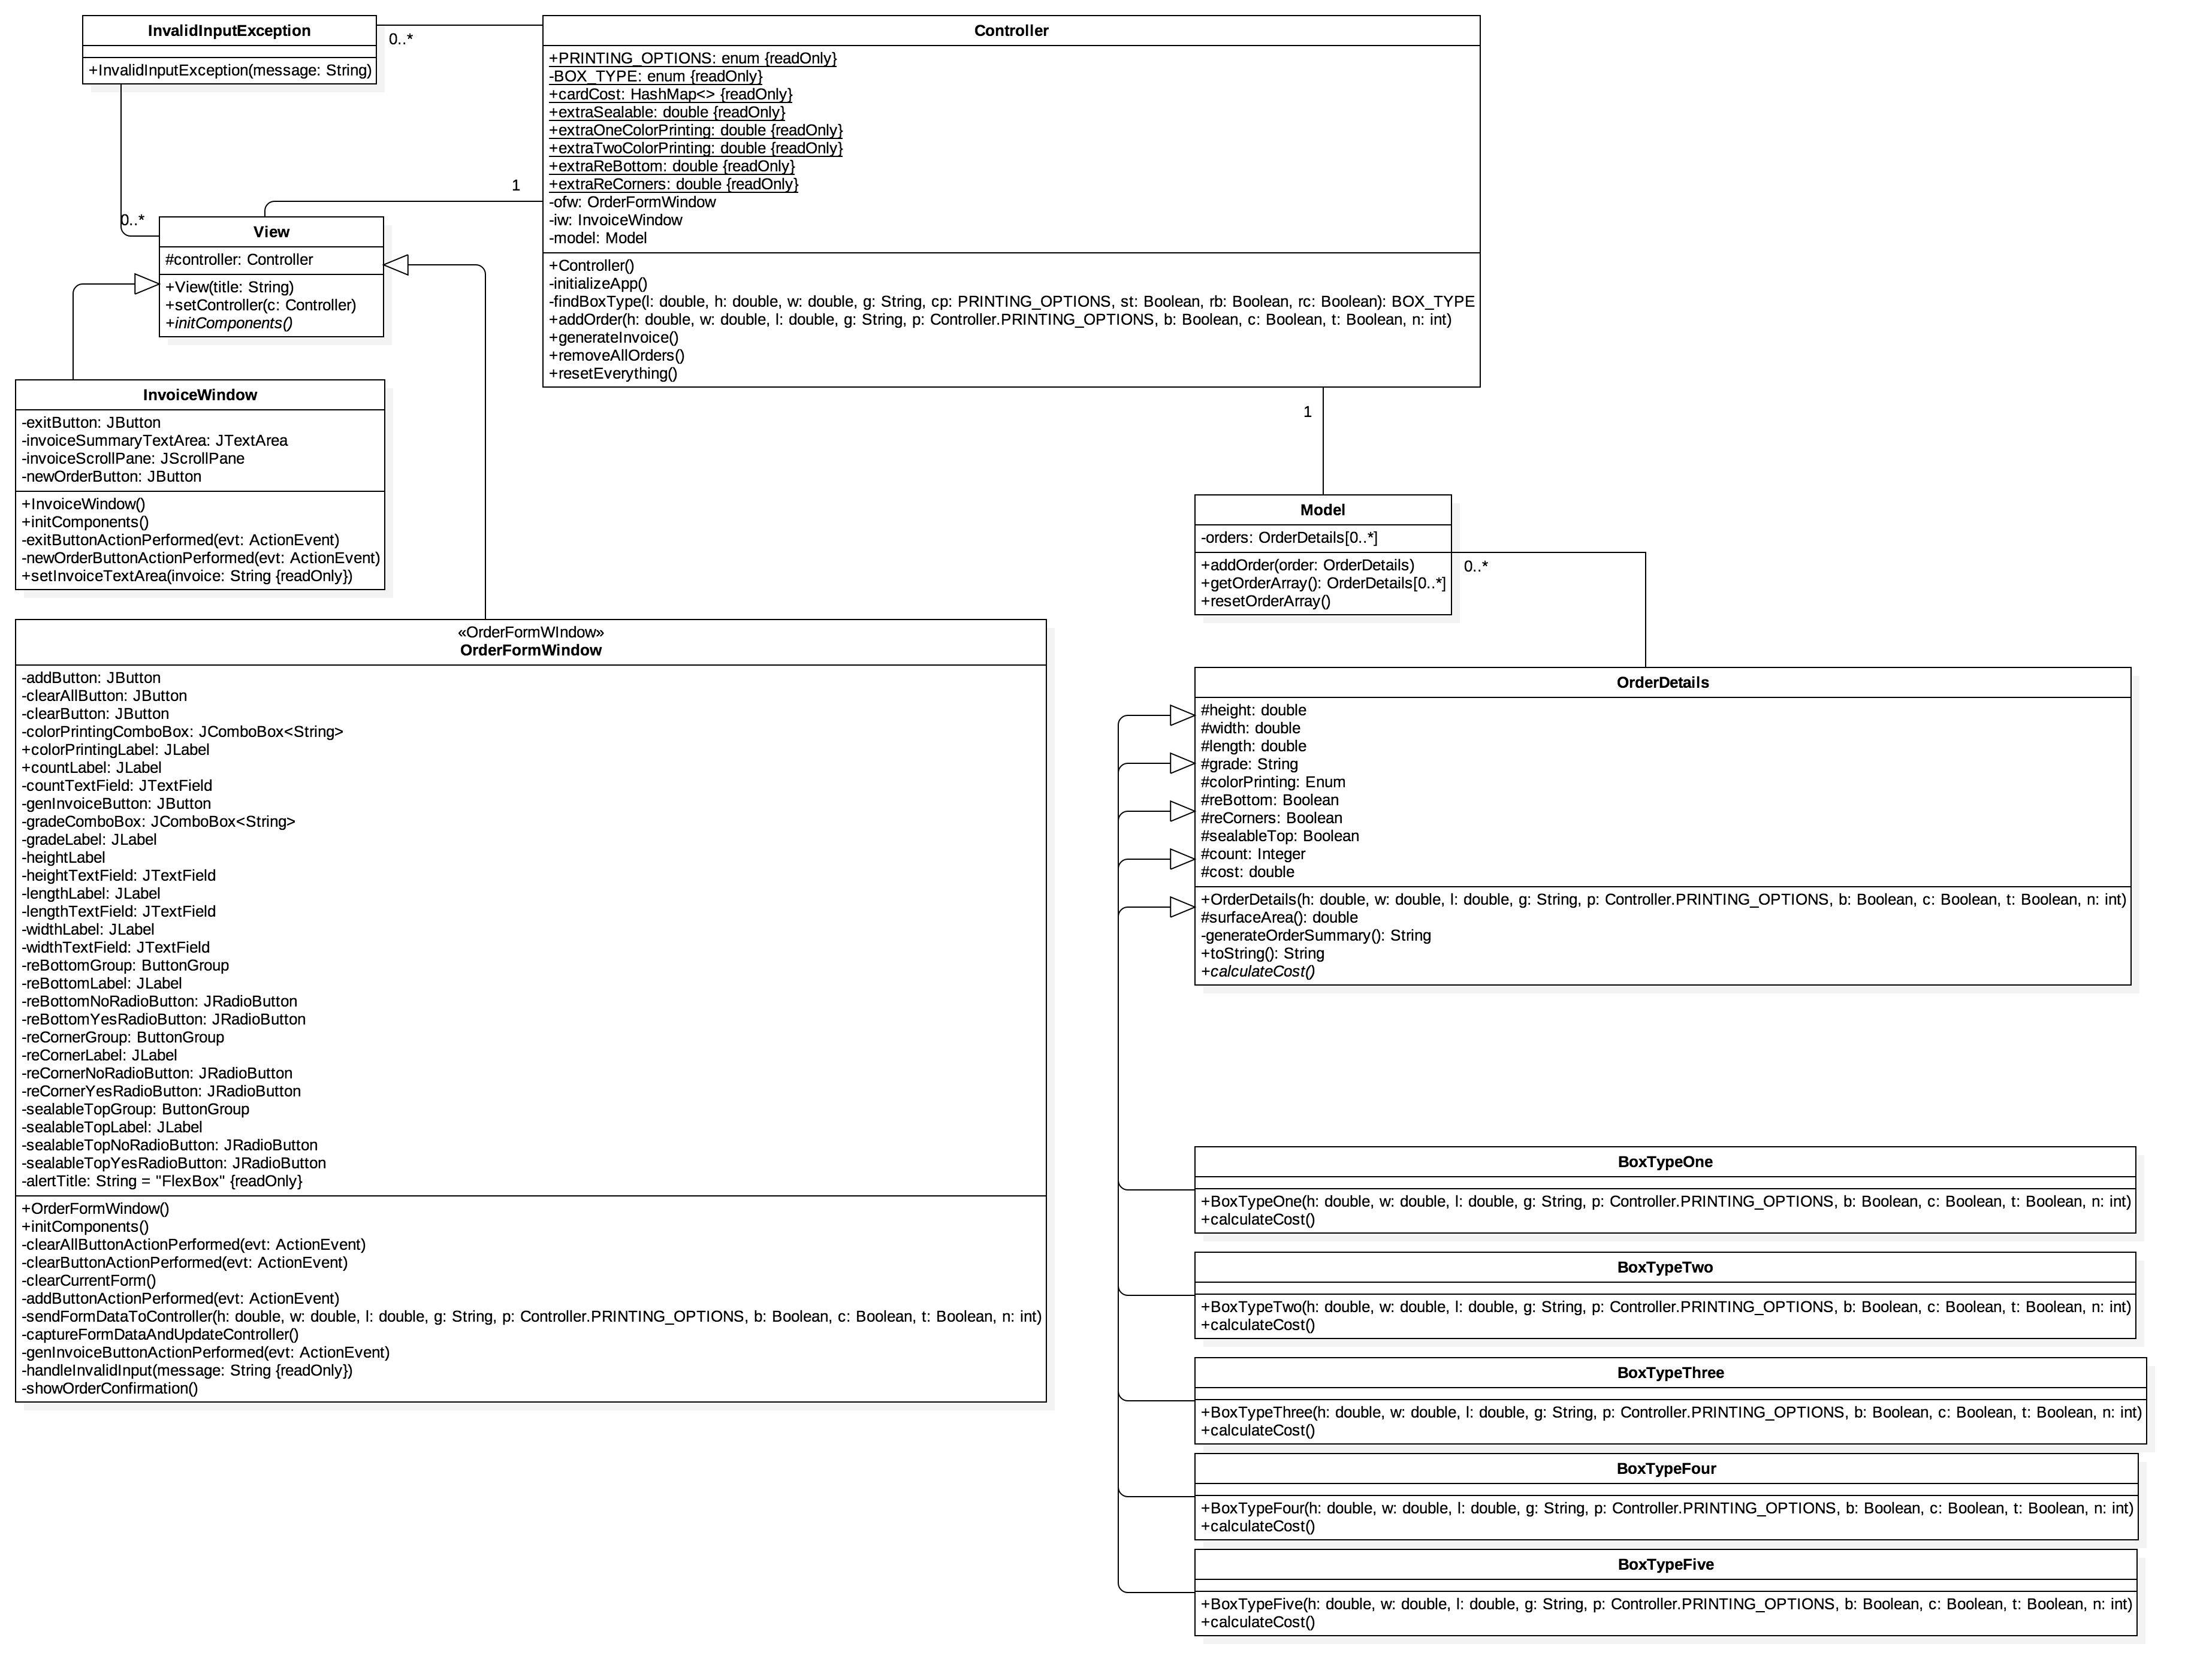
\includegraphics[scale=0.13]{./diagrams/ClassHierarchyDiagram.jpg}
\subsection{Instance Diagram}
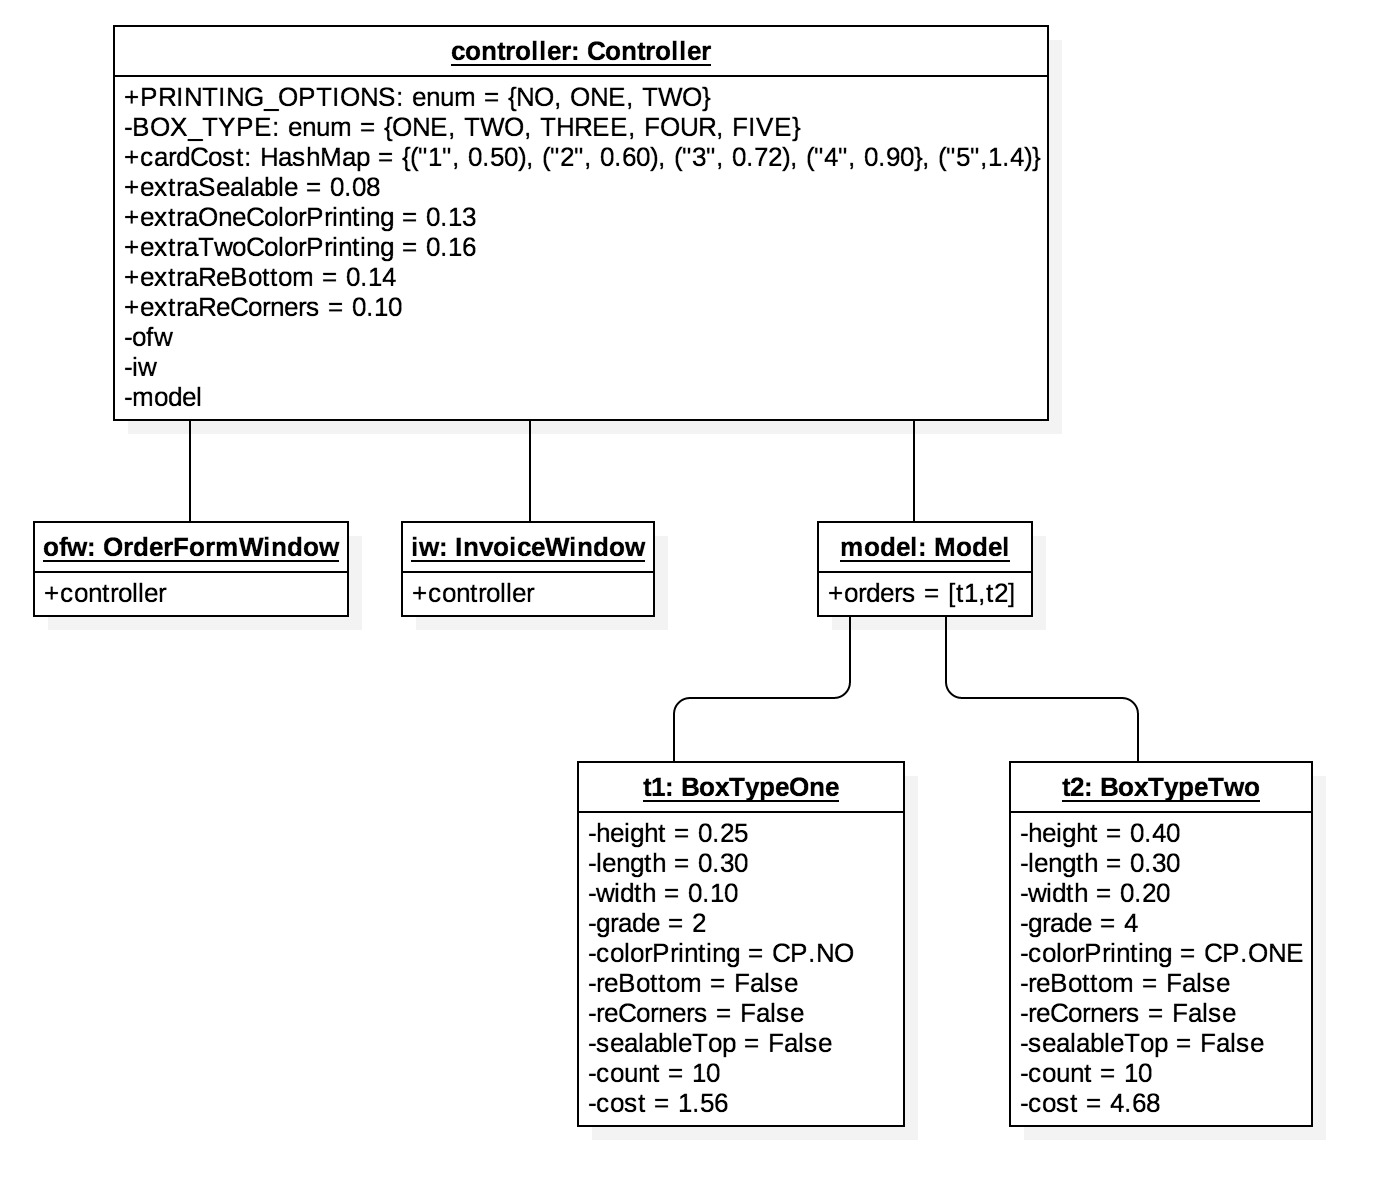
\includegraphics[scale=.3]{./diagrams/InstanceDiagram.jpg}
\subsection{Use Case Diagram}
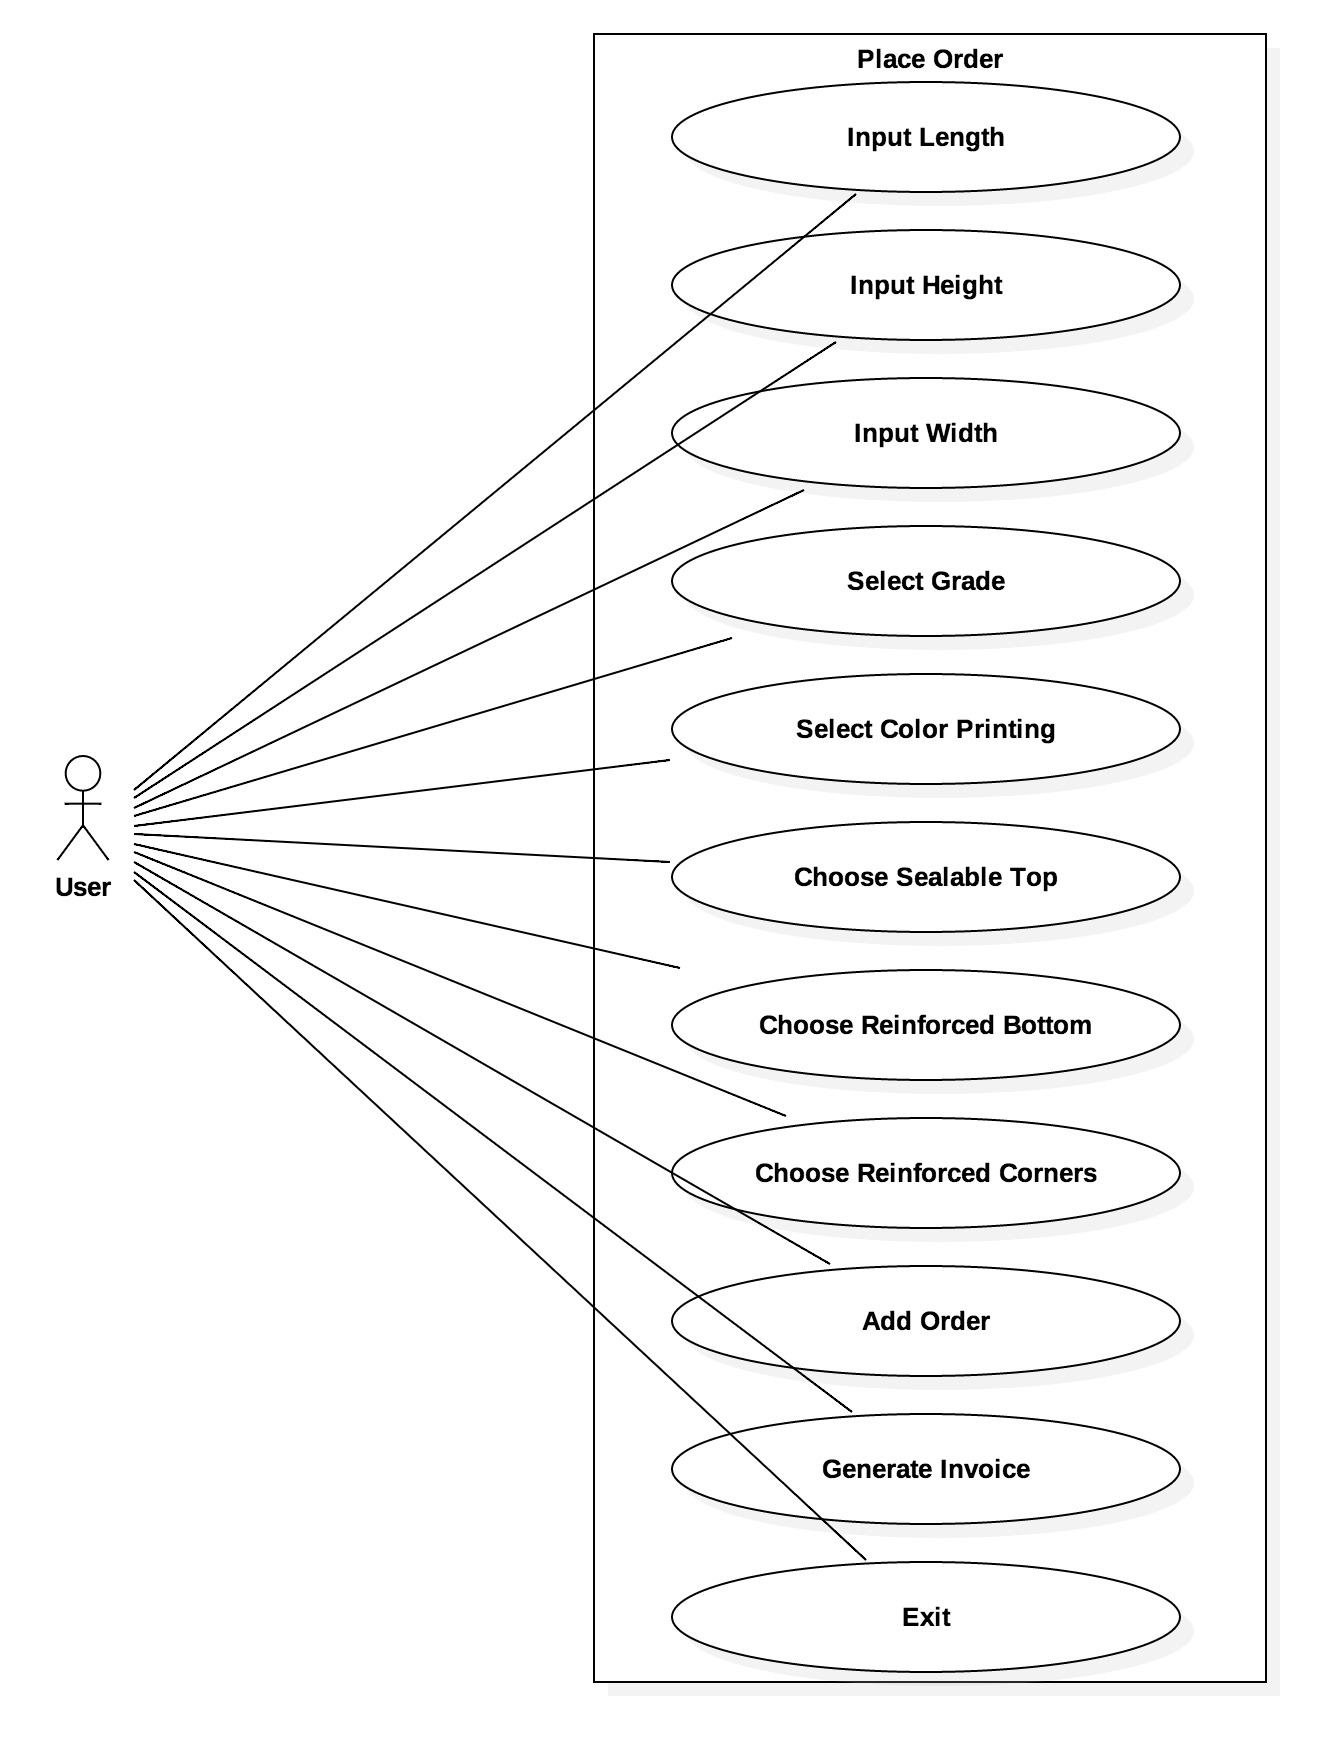
\includegraphics[scale=.30]{./diagrams/UseCaseDiagram.jpg}
\subsection{Sequence Diagram}
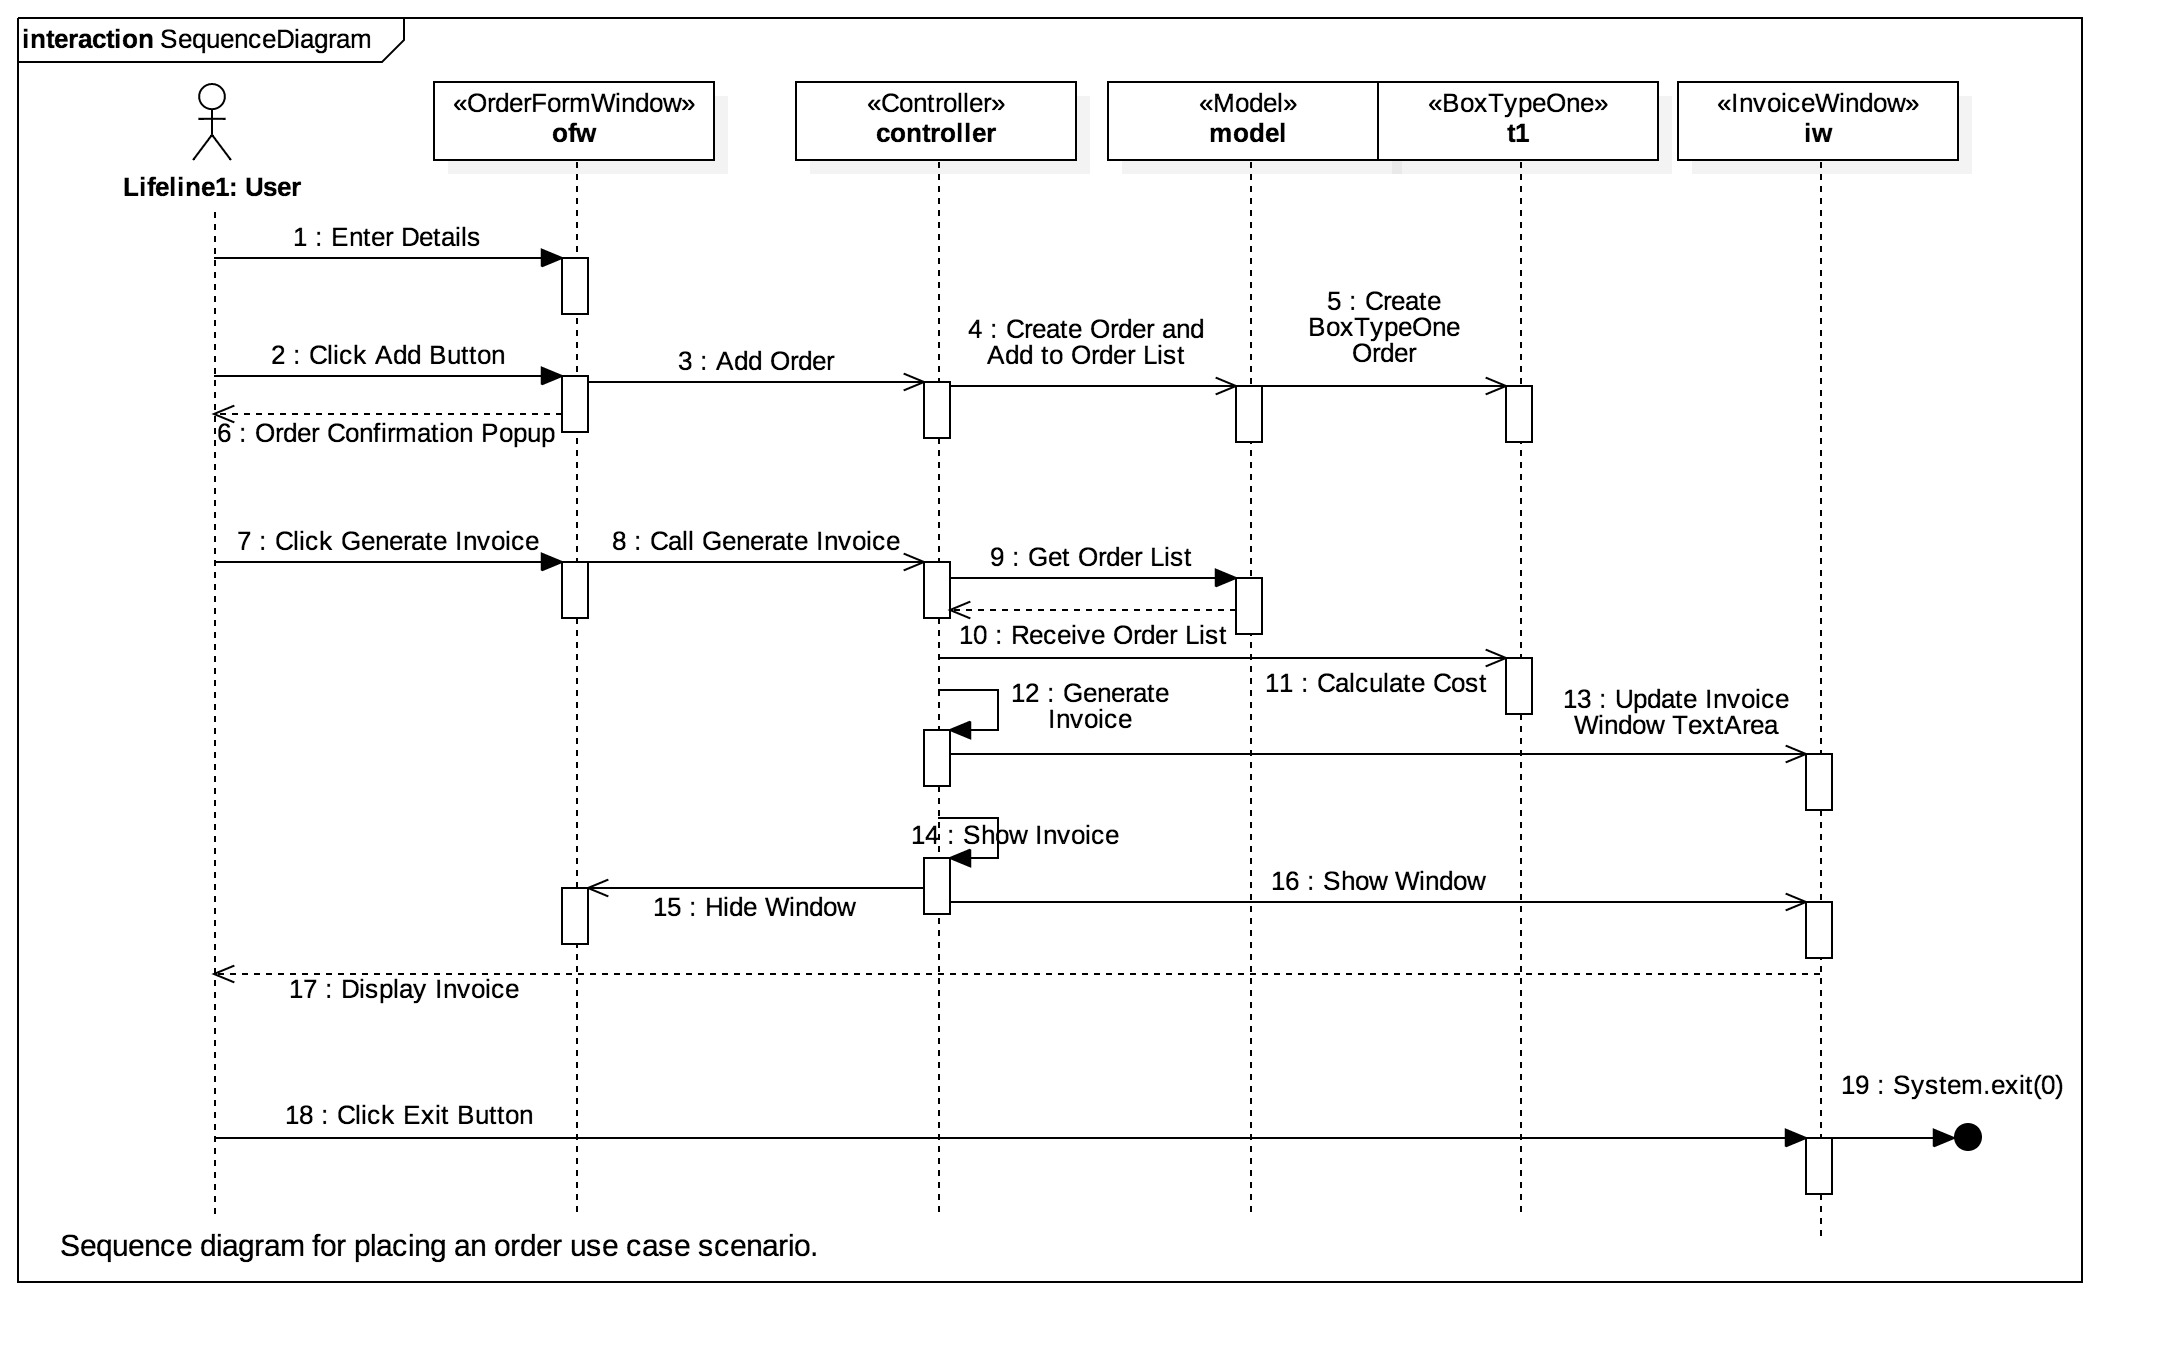
\includegraphics[scale=.20]{./diagrams/SequenceDiagram.jpg}
\newpage
\section{Test Schedule}
\begin{tabular}{| p{1cm} | p{4cm} | p{4cm} | p{4cm} | p{2cm} |}
	\hline
	\textbf{No} & \textbf{Test Case} & \textbf{Input} & \textbf{Expected Output} & \textbf{Status} \\ \hline
	1 & Invalid input(s) & Length: a \newline
	Height: .25 \newline
	Width: .30 \newline
	Number of Boxes: 10 & A popup showing error message "Invalid input: Please check the values" & Pass \\ \hline
	2 & Incorrect input(s) & Length: 0.20 \newline
	Height: 0.30 \newline
	Widht: 0.25 \newline
	Number of Boxes: 0 & A popup showing error message "Invalid input: Box dimensions and count must be greater than 0" & Pass \\ \hline
	3 & Non-suppliable order & Length: .10 \newline
	Height: .20 \newline
	Width: .40 \newline
	Grade: 4 \newline
	Reinforced Bottom: Yes \newline
	Number of Boxes: 10 & A popup showing error message "Sorry, we are not able to supply this order" & Pass \\ \hline
	4 & Generate invoice for empty order list & Click 'Generate Invoice' button without adding any orders. & A popup showing error message "Please add your order before generating the invoice" & Pass \\ \hline
	5 & Single Order invoice & Length: 0.20 \newline
	Height: 0.30 \newline
	Width: 0.25 \newline
	Grade: 3 \newline
	Color Printing: TWO COLORS \newline
	Reinforced Bottom: Yes \newline
	Reinforced Corner: Yes \newline
	Sealable Top: No \newline
	Number of Boxes: 10 & A popup showing info message "Order added successfully". \newline Invoice for the order. & Pass \\ \hline
\end{tabular}
\newpage
\begin{tabular}{| p{1cm} | p{4cm} | p{4cm} | p{4cm} | p{2cm} |}
	\hline
	6 & Multiple orders in same invoice & \textbf{Order 1} \newline
	Length: 0.20 \newline
	Height: 0.30 \newline
	Widht: 0.25 \newline
	Grade: 3 \newline
	Color Printing: TWO COLORS \newline
	Reinforced Bottom: Yes \newline
	Reinforced Corner: No \newline
	Sealable Top: No \newline
	Number of Boxes: 15 \newline
	\newline
	\textbf{Order 2} \newline
	Length: 0.25 \newline
	Height: 0.30 \newline
	Widht: 0.15 \newline
	Grade: 5 \newline
	Color Printing: TWO COLORS \newline
	Reinforced Bottom: Yes \newline
	Reinforced Corner: Yes \newline
	Sealable Top: No \newline
	Number of Boxes: 10 \newline
	\newline
	\textbf{Order 3} \newline
	Length: 0.20 \newline
	Height: 0.30 \newline
	Widht: 0.25 \newline
	Grade: 1 \newline
	Color Printing: NO COLORS \newline
	Reinforced Bottom: No \newline
	Reinforced Corner: No \newline
	Sealable Top: Yes \newline
	Number of Boxes: 20 & A "Order added successfully" popup for each oder.\newline
	Single invoice for all the three orders. & Pass \\ \hline
\end{tabular}
\subsection{Screenshots}
\begin{figure}[H]
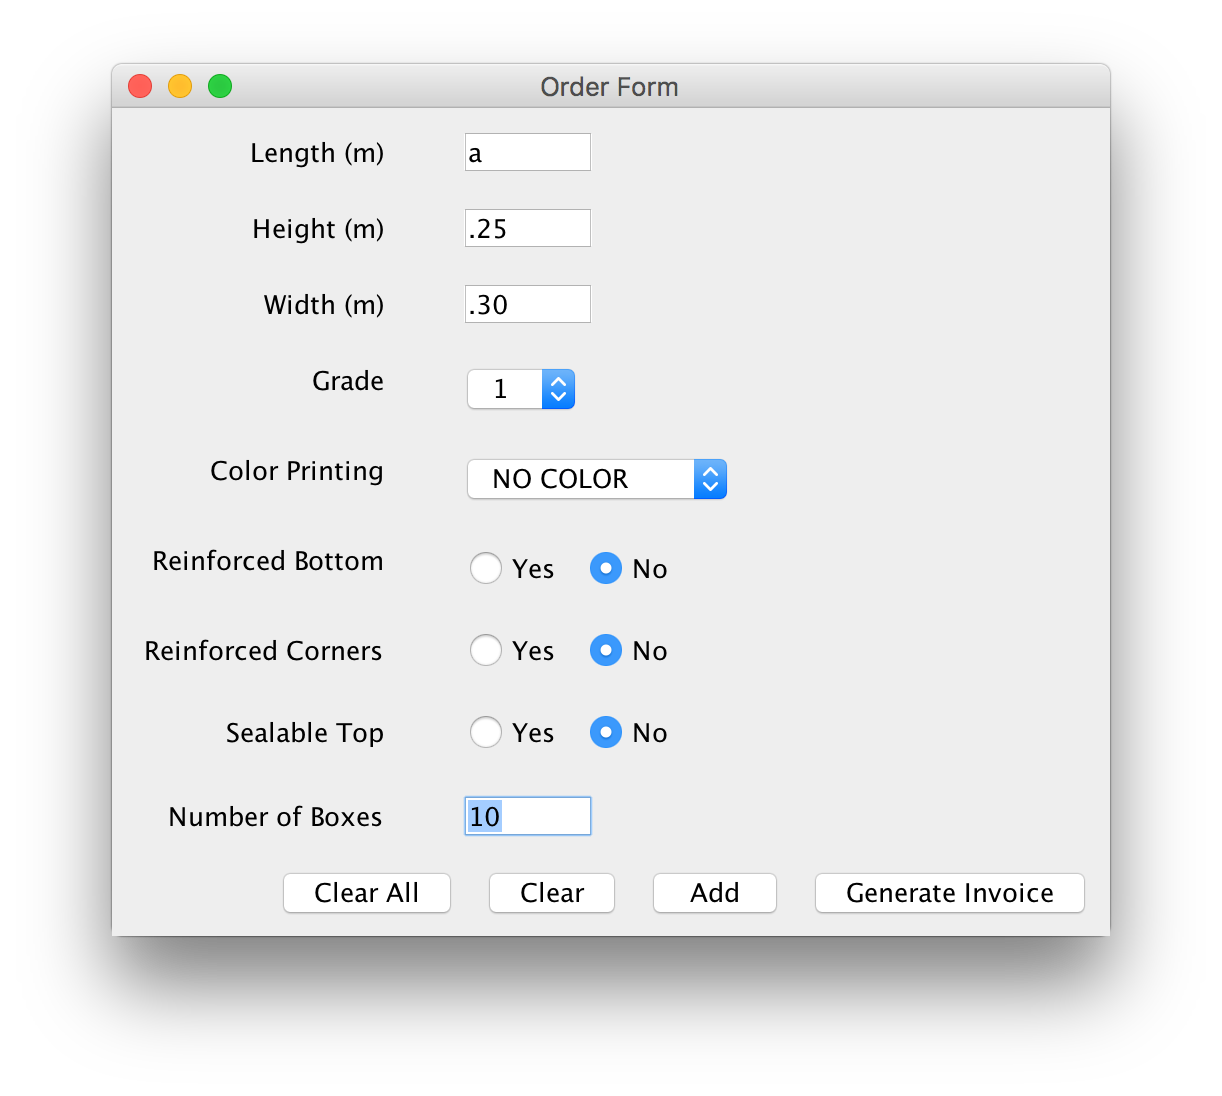
\includegraphics[width=\linewidth]{./screenshots/test_case_1_input.png}
\caption{Test Case 1 Input}
\label{test_case_1_input}
\end{figure}
\begin{figure}[H]
	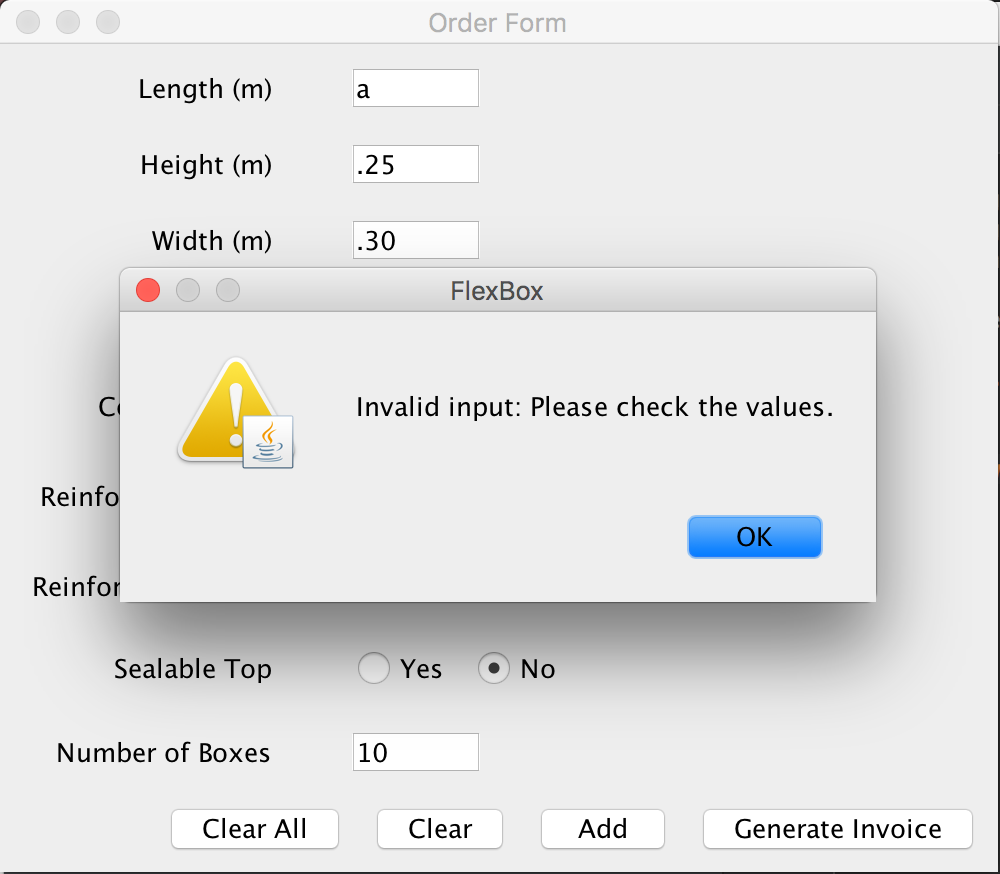
\includegraphics[width=\linewidth]{./screenshots/test_case_1_output.png}
	\caption{Test Case 1 Output}
	\label{test_case_1_output}
\end{figure}
\begin{figure}[H]
	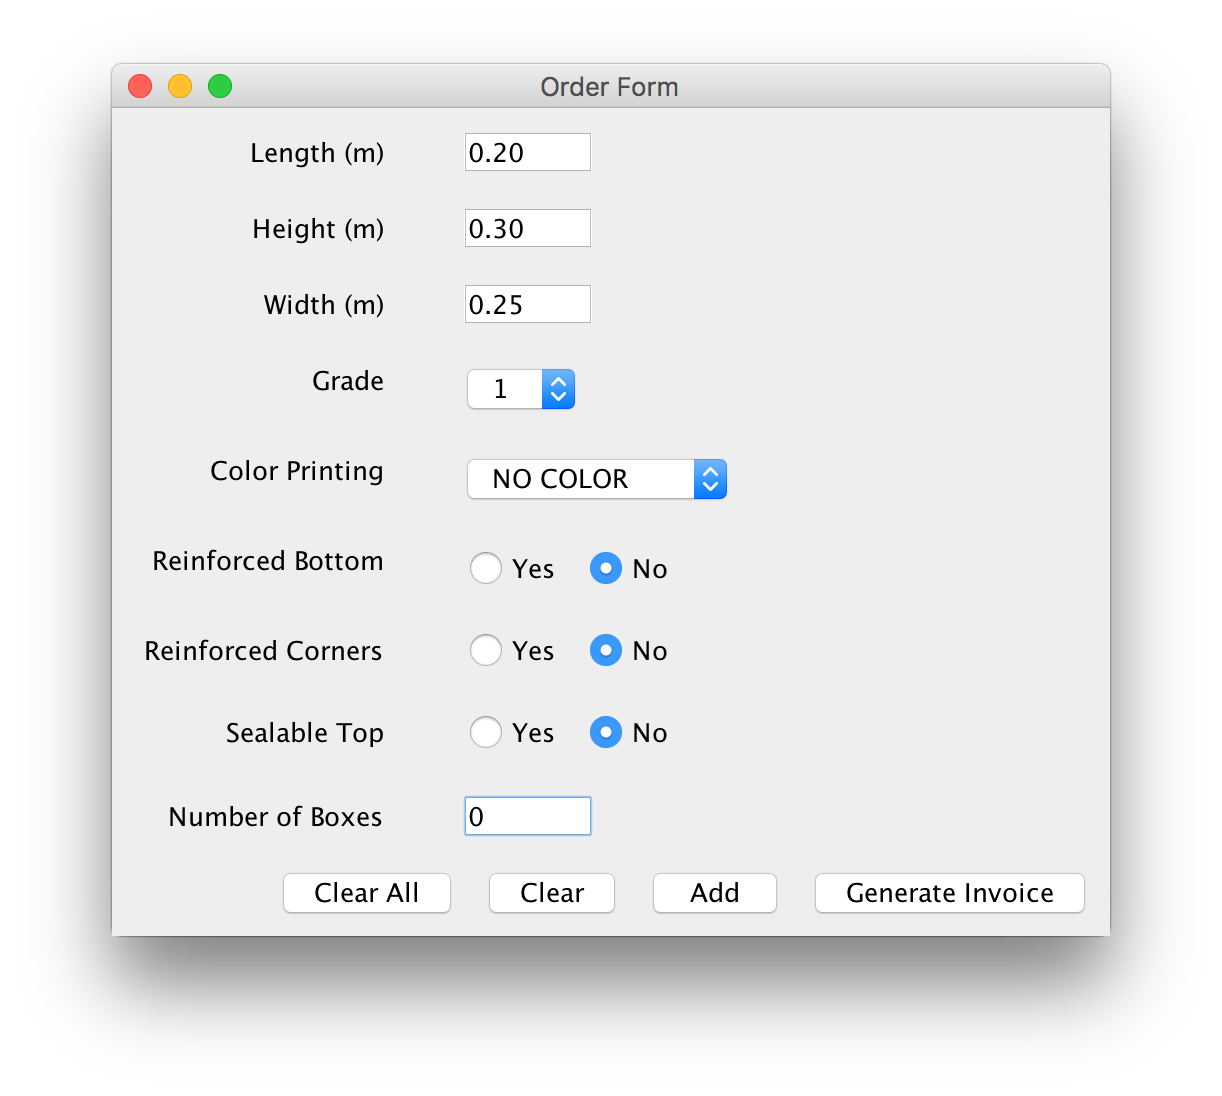
\includegraphics[width=\linewidth]{./screenshots/test_case_2_input.png}
	\caption{Test Case 2 Input}
	\label{test_case_2_input}
\end{figure}
\begin{figure}[H]
	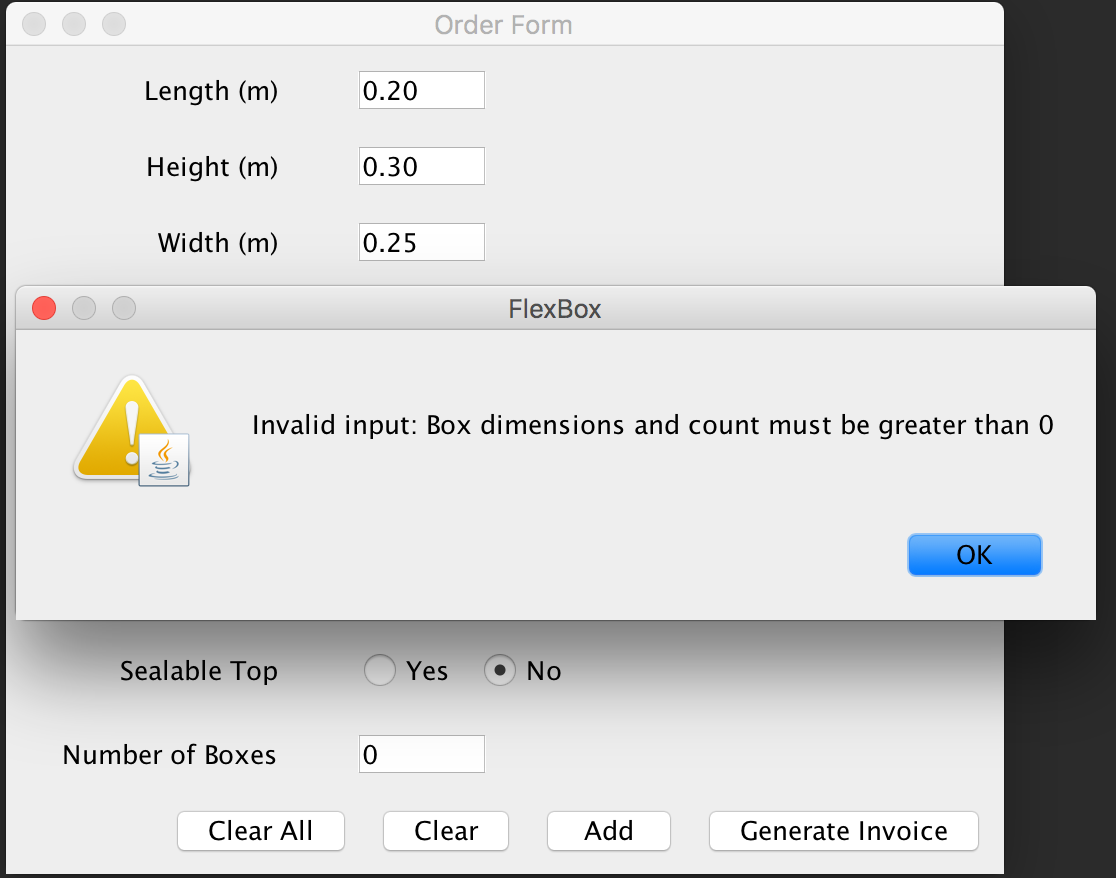
\includegraphics[width=\linewidth]{./screenshots/test_case_2_output.png}
	\caption{Test Case 2 Output}
	\label{test_case_2_output}
\end{figure}
\begin{figure}[H]
	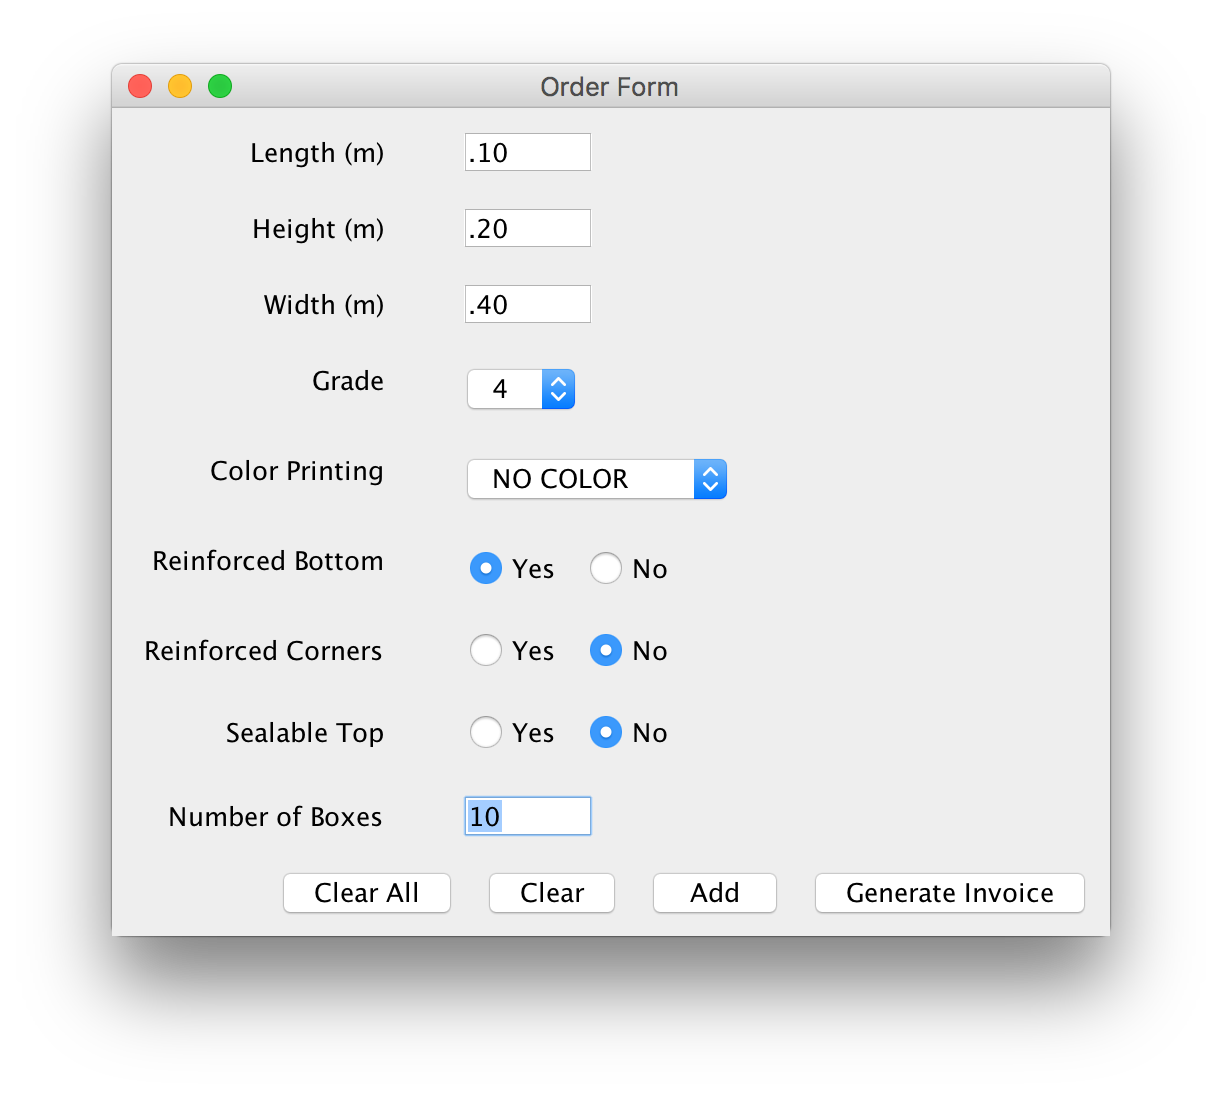
\includegraphics[width=\linewidth]{./screenshots/test_case_3_input.png}
	\caption{Test Case 3 Input}
	\label{test_case_3_input}
\end{figure}
\begin{figure}[H]
	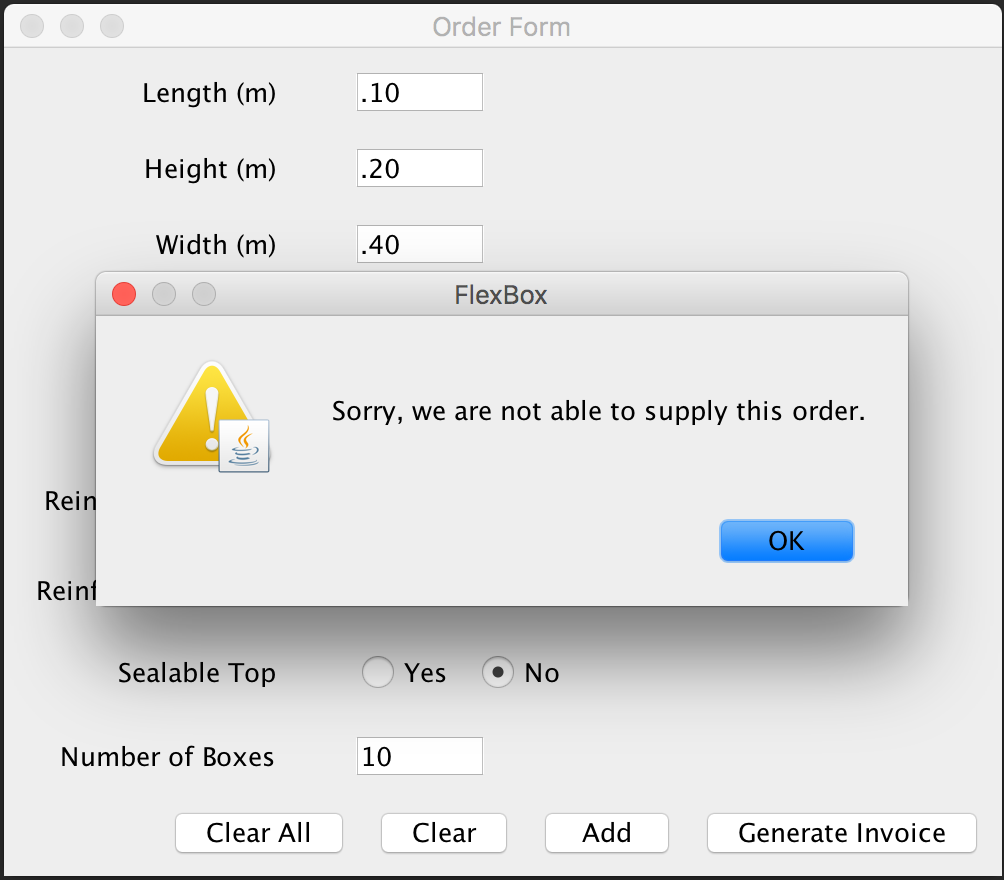
\includegraphics[width=\linewidth]{./screenshots/test_case_3_output.png}
	\caption{Test Case 3 Output}
	\label{test_case_3_output}
\end{figure}
\begin{figure}[H]
	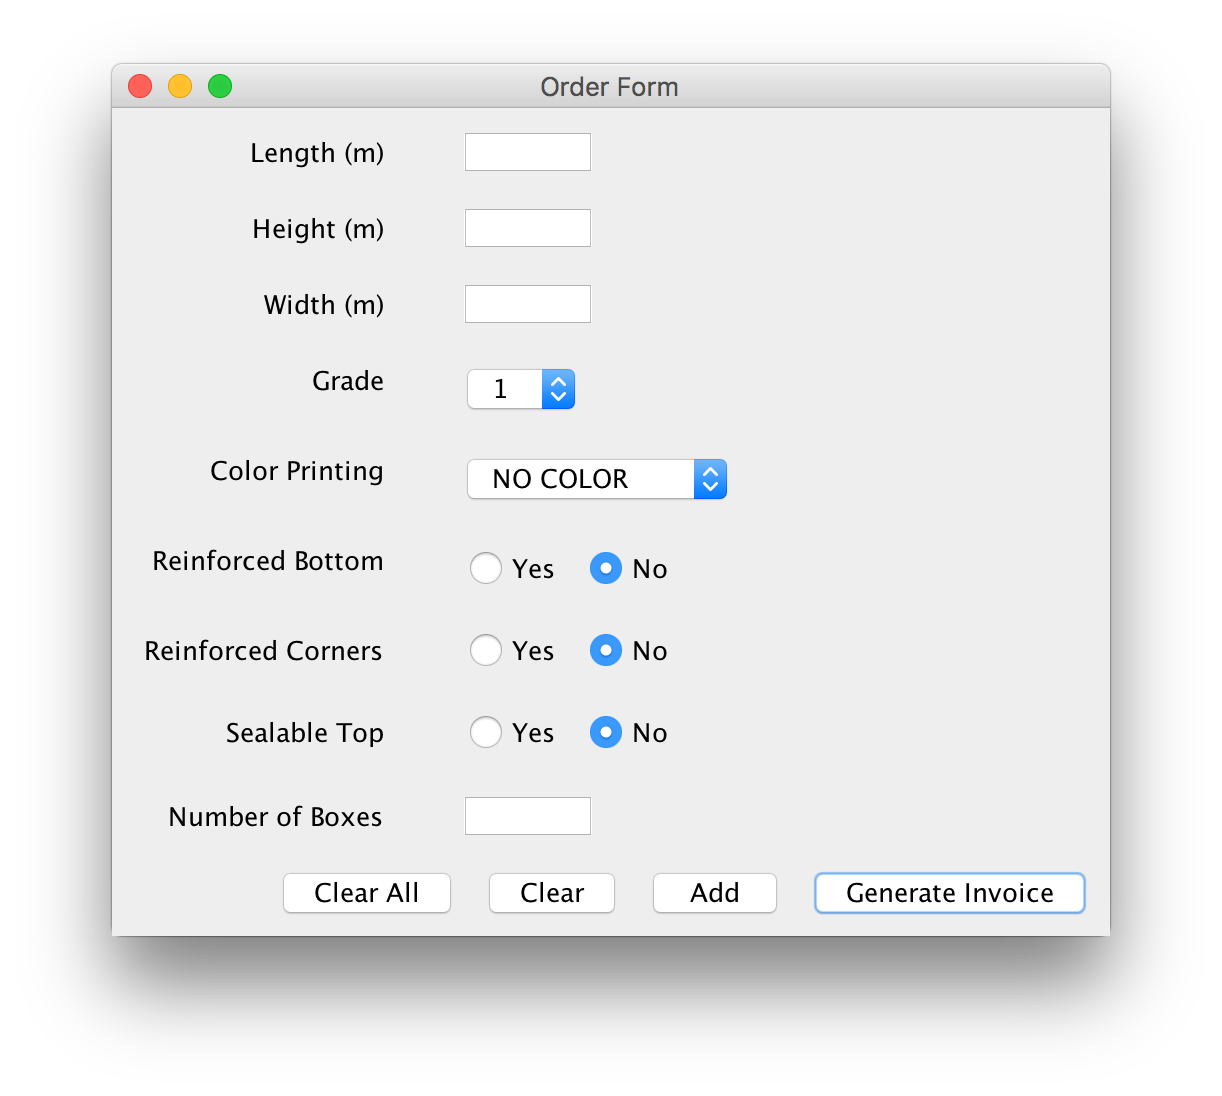
\includegraphics[width=\linewidth]{./screenshots/test_case_4_input.png}
	\caption{Test Case 4 Input}
	\label{test_case_4_input}
\end{figure}
\begin{figure}[H]
	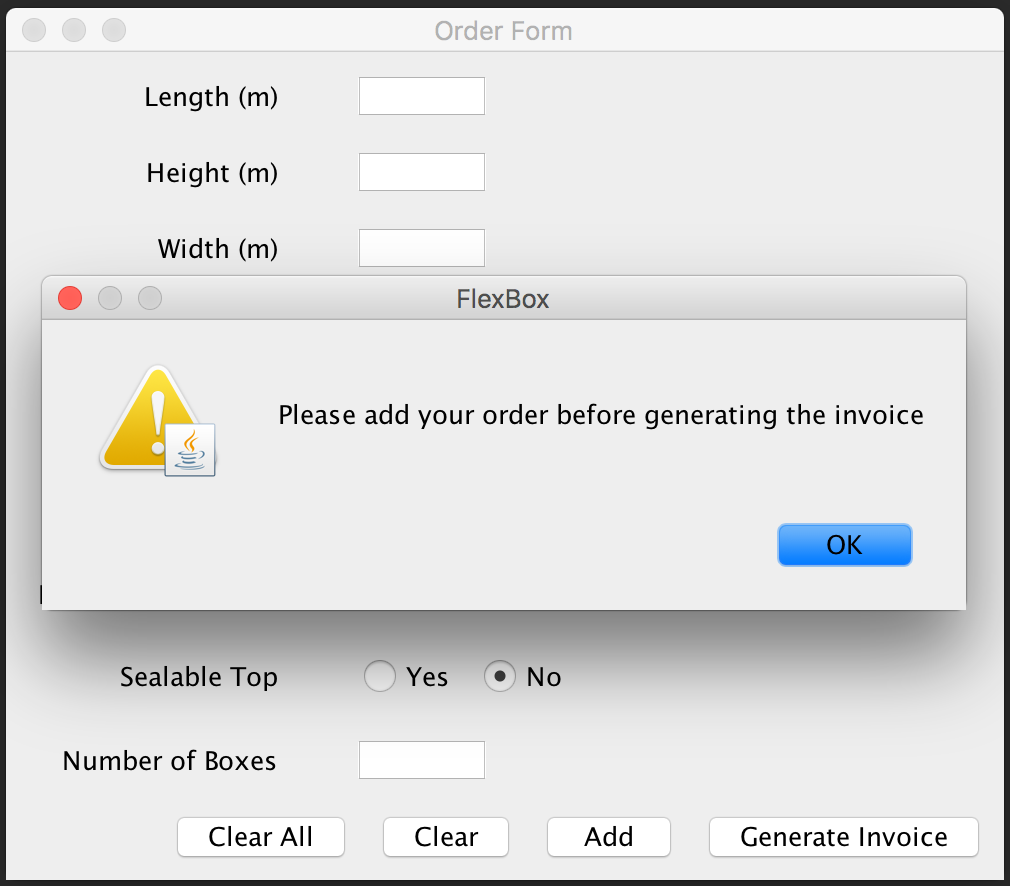
\includegraphics[width=\linewidth]{./screenshots/test_case_4_output.png}
	\caption{Test Case 4 Output}
	\label{test_case_4_output}
\end{figure}
\begin{figure}[H]
	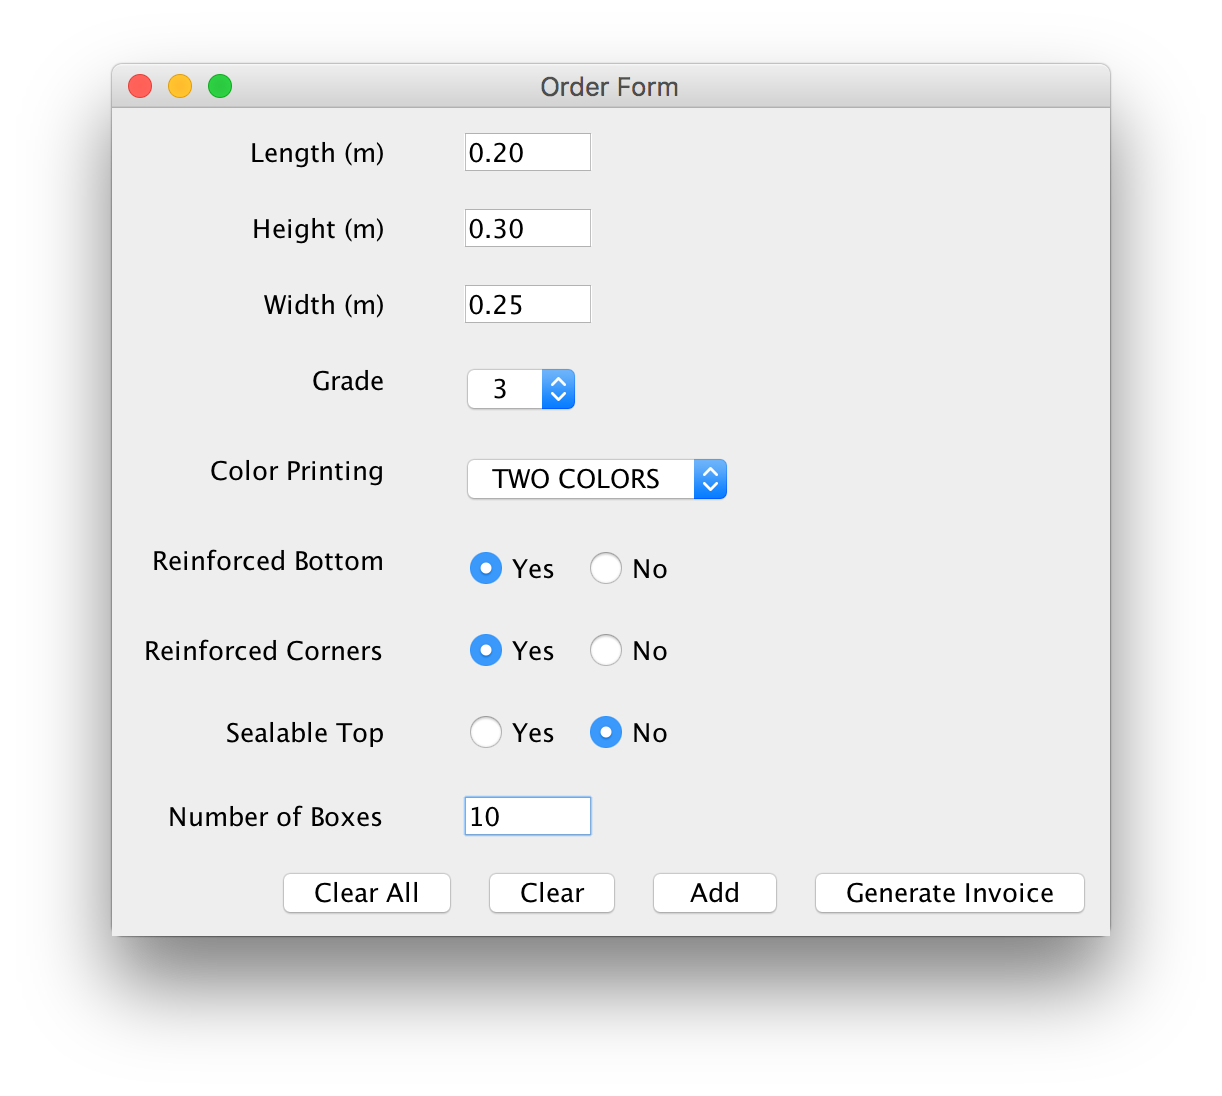
\includegraphics[width=\linewidth]{./screenshots/test_case_5_input.png}
	\caption{Test Case 5 Input}
	\label{test_case_5_input}
\end{figure}
\begin{figure}[H]
	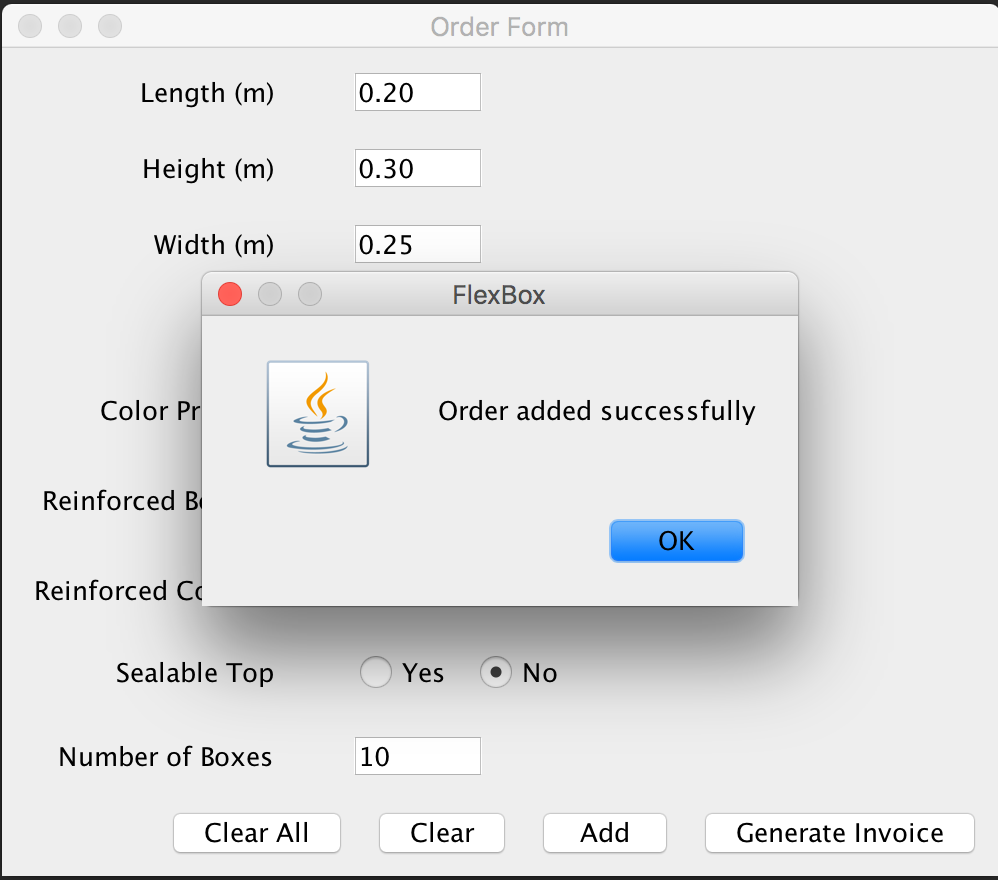
\includegraphics[width=\linewidth]{./screenshots/test_case_5_output_1.png}
	\caption{Test Case 5 Output 1}
	\label{test_case_5_output}
\end{figure}
\begin{figure}[H]
	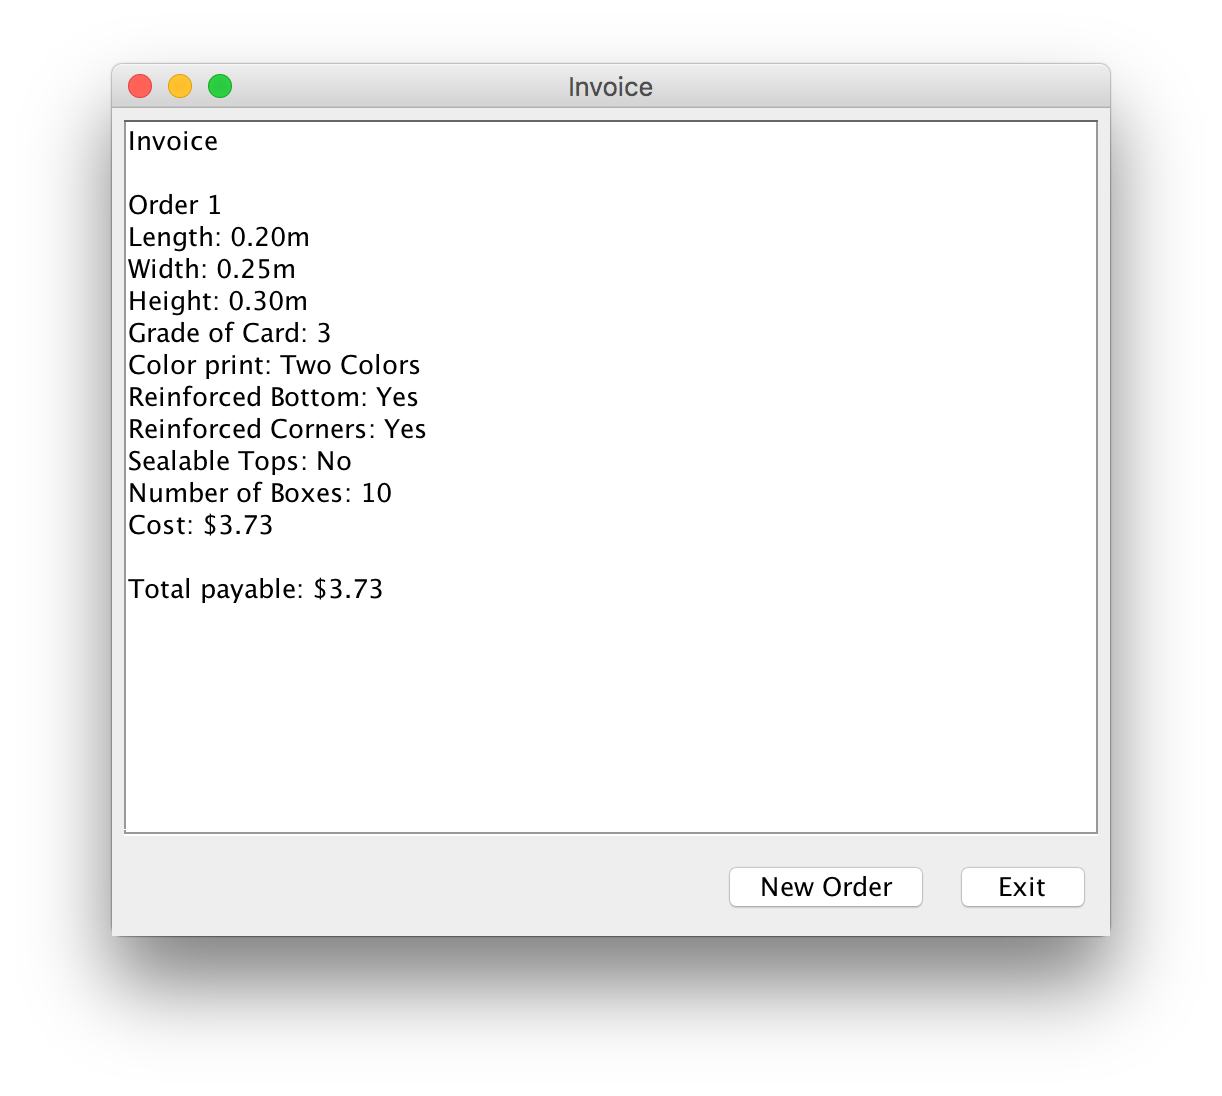
\includegraphics[width=\linewidth]{./screenshots/test_case_5_output_2.png}
	\caption{Test Case 5 Output 2}
	\label{test_case_5_output}
\end{figure}
\begin{figure}[H]
	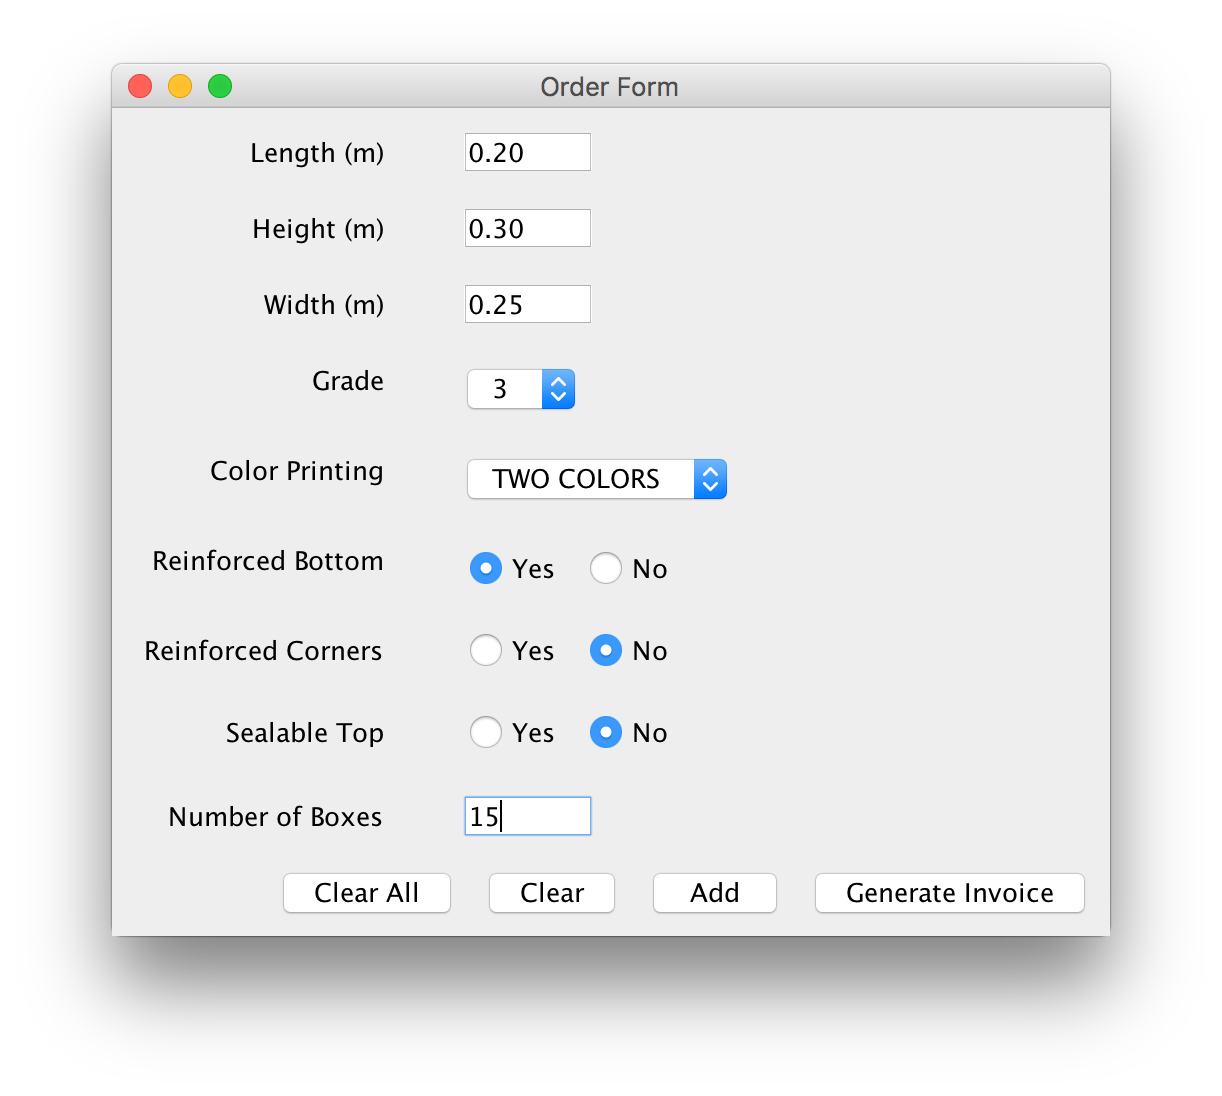
\includegraphics[width=\linewidth]{./screenshots/test_case_6_order1_input.png}
	\caption{Test Case 6 Input 1}
	\label{test_case_6_input_1}
\end{figure}
\begin{figure}[H]
	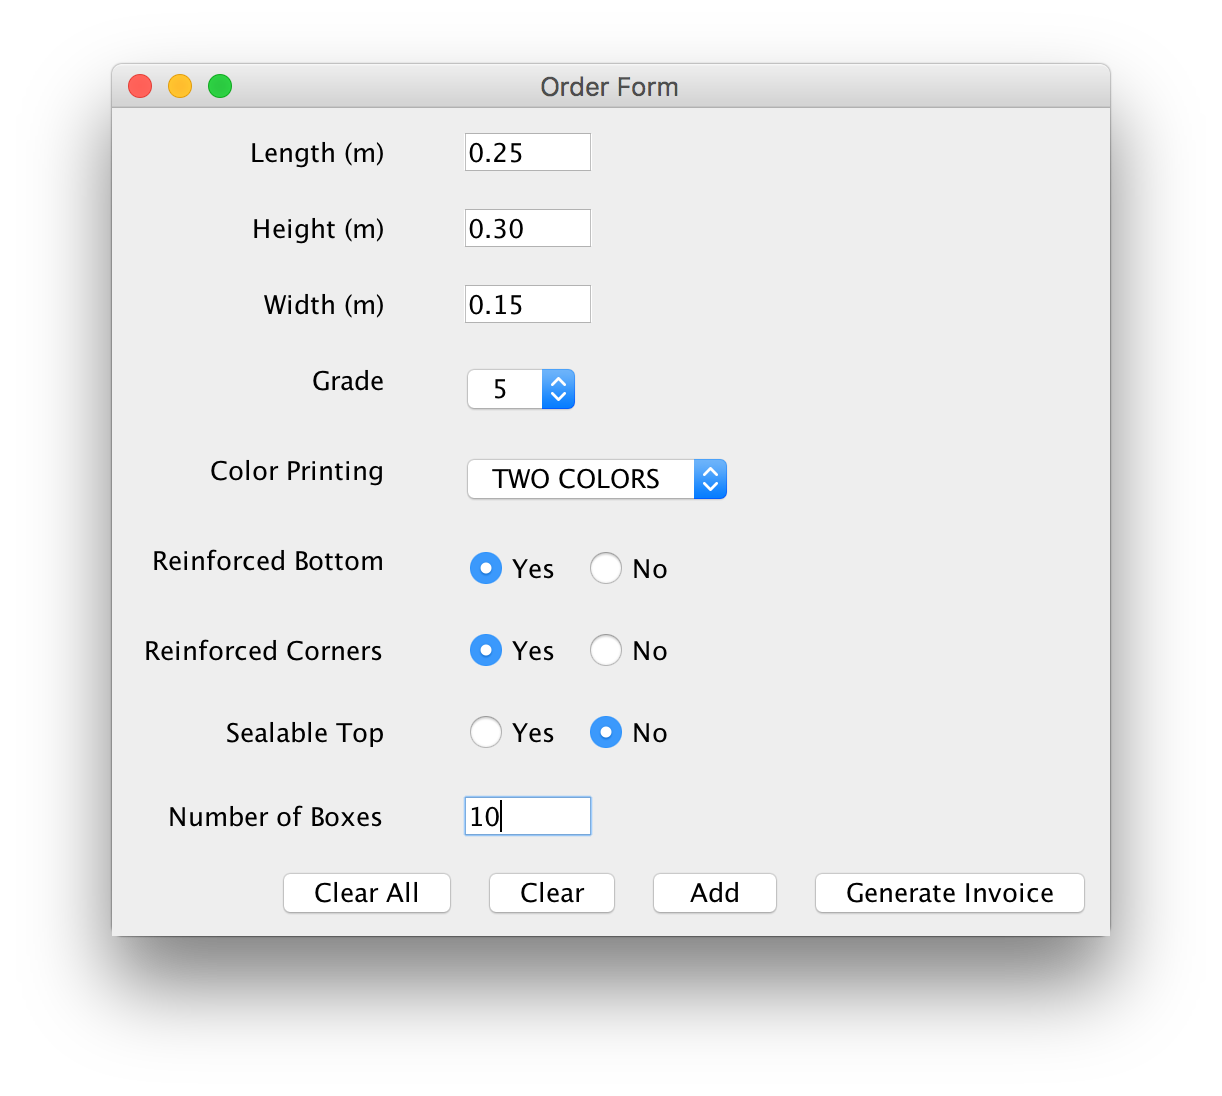
\includegraphics[width=\linewidth]{./screenshots/test_case_6_order2_input.png}
	\caption{Test Case 6 Input 2}
	\label{test_case_6_input_2}
\end{figure}
\begin{figure}[H]
	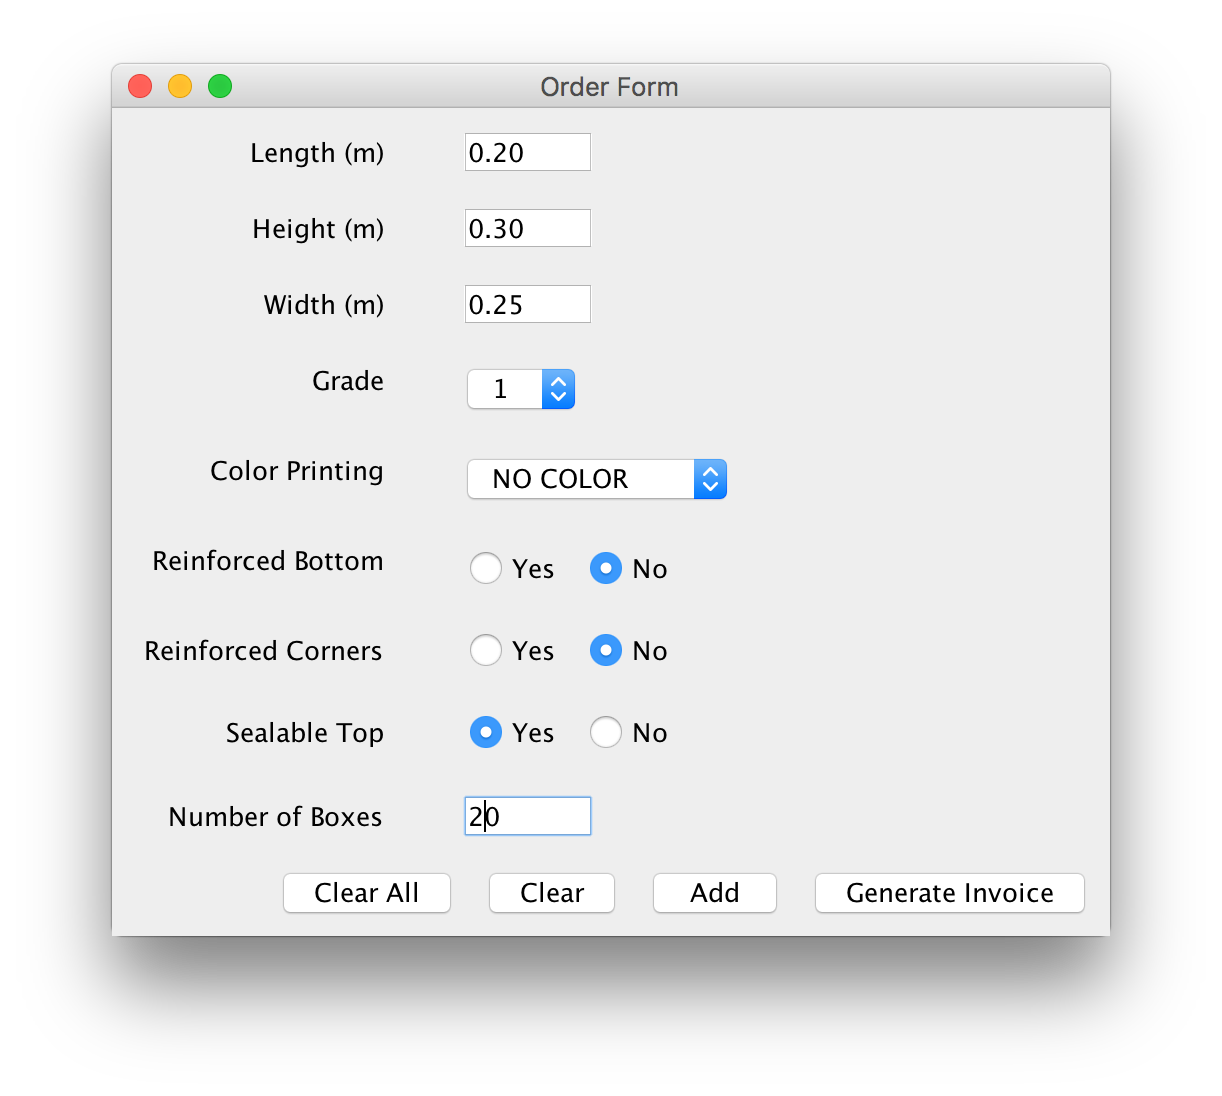
\includegraphics[width=\linewidth]{./screenshots/test_case_6_order3_input.png}
	\caption{Test Case 6 Input 3}
	\label{test_case_6_input_3}
\end{figure}
\begin{figure}[H]
	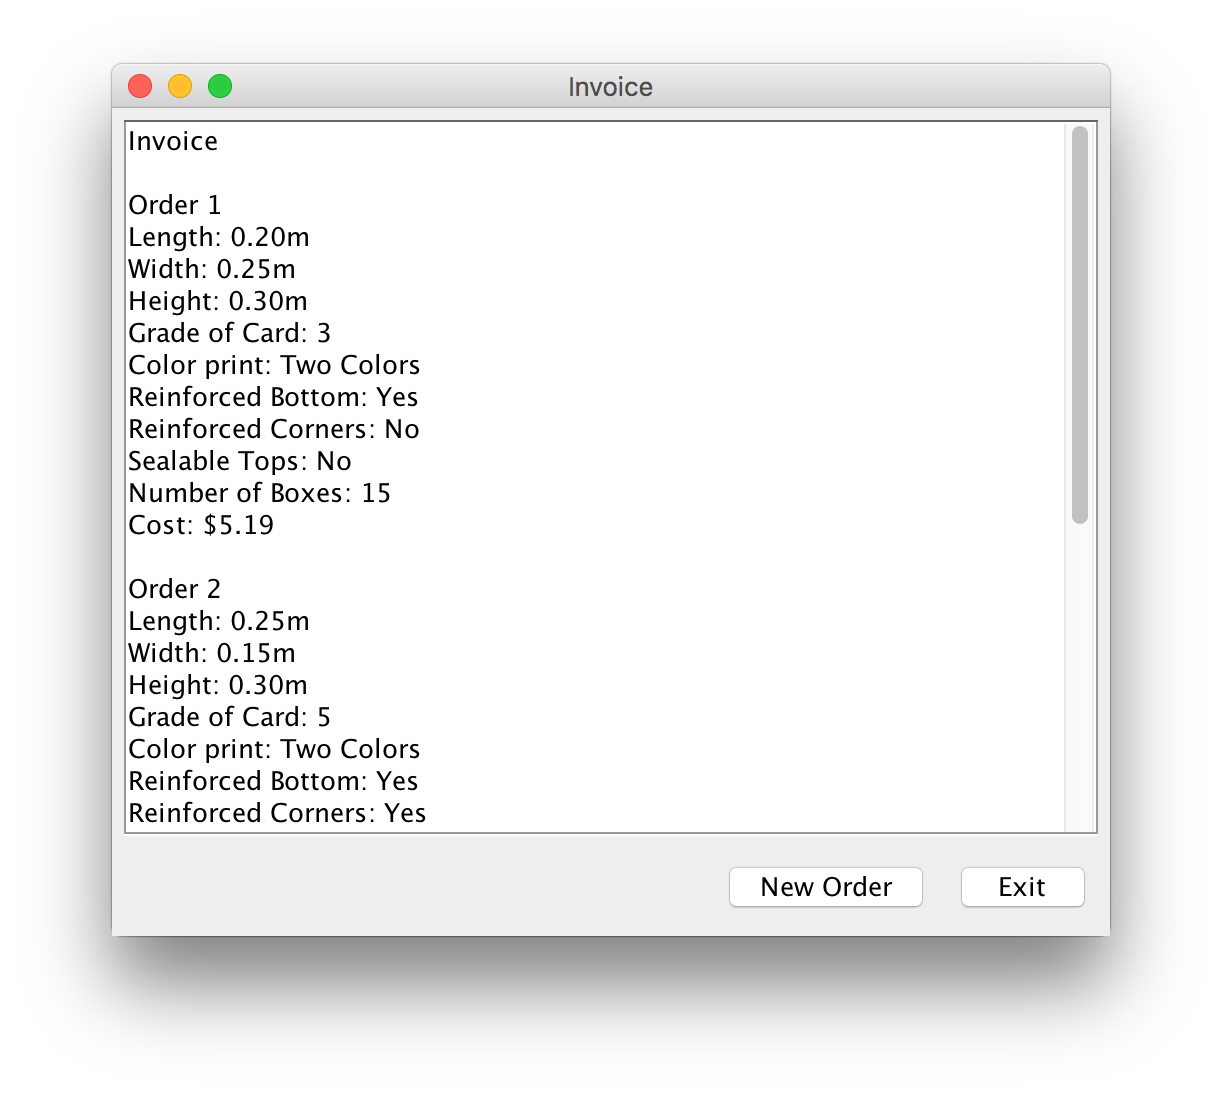
\includegraphics[width=\linewidth]{./screenshots/test_case_6_output_part1.png}
	\caption{Test Case 6 Output Part 1}
	\label{test_case_6_output}
\end{figure}
\begin{figure}[H]
	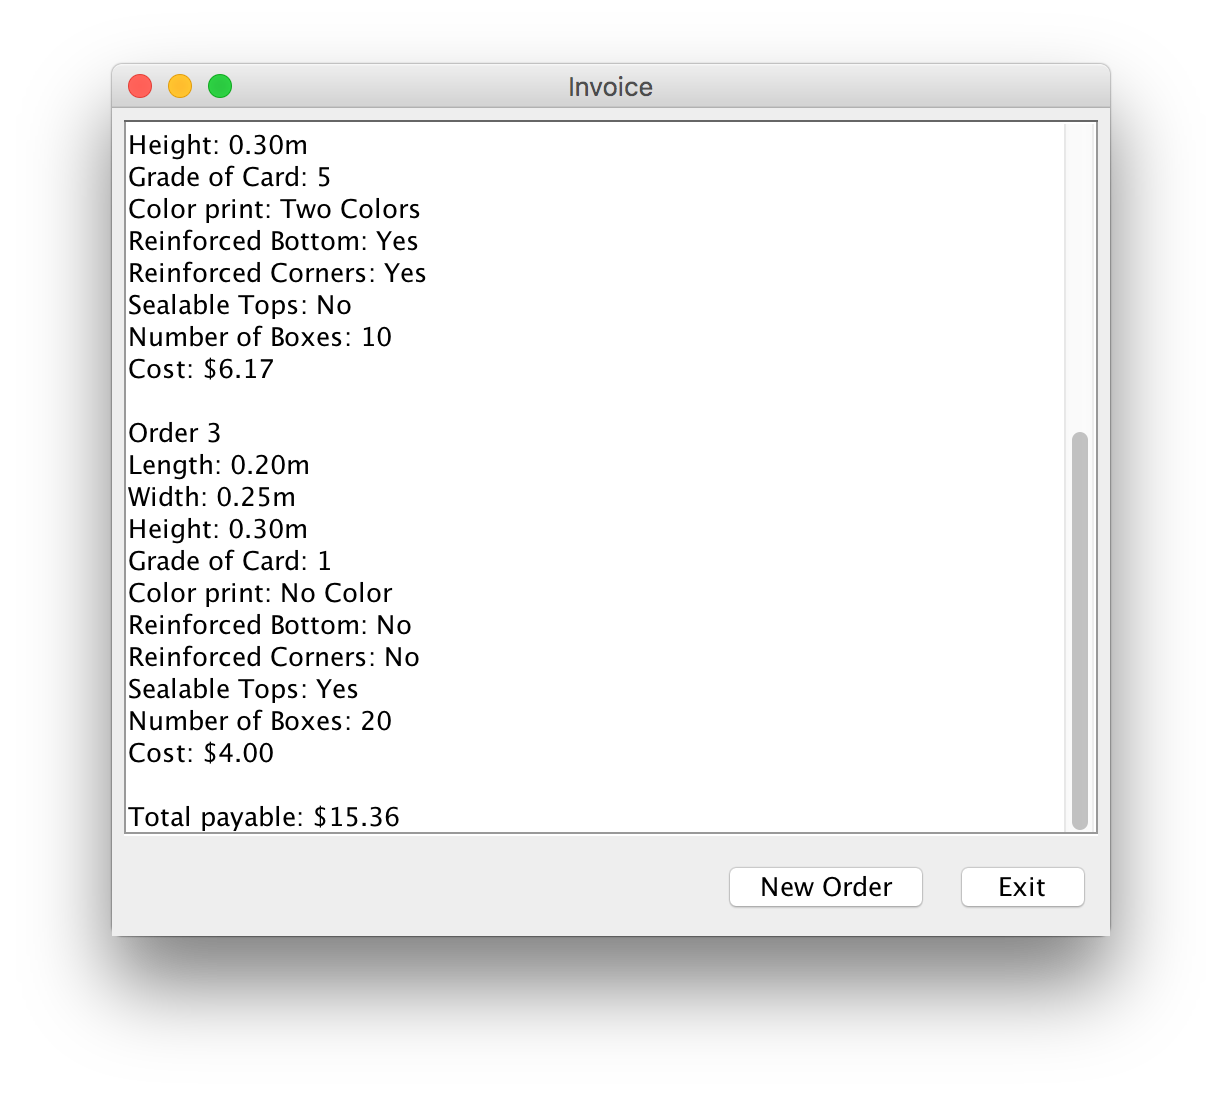
\includegraphics[width=\linewidth]{./screenshots/test_case_6_output_part2.png}
	\caption{Test Case 6 Output Part 2}
	\label{test_case_6_output}
\end{figure}
\newpage
\section{Sample Inputs and Outputs}
\begin{tabular}{| p{1cm} | p{6cm} | p{6cm} |}
	\hline
	\textbf{No} & \textbf{Input} & \textbf{Output} \\ \hline
	1 & Length: 0.25\newline
	Height: 0.30\newline
	Width: 0.20\newline
	Grade: 2\newline
	Color Printing: ONE COLOR\newline
	Reinforcement Bottom: No\newline
	Reinforcement Corners: No\newline
	Sealable Top: Yes\newline
	Number of Boxes: 10 & Invoice\newline
	\newline
	Order 1\newline
	Length: 0.25m\newline
	Width: 0.20m\newline
	Height: 0.30m\newline
	Grade of Card: 2\newline
	Color print: No Color\newline
	Reinforced Bottom: No\newline
	Reinforced Corners: No\newline
	Sealable Tops: Yes\newline
	Number of Boxes: 10\newline
	Cost: \$2.40\newline
	\newline
	Total payable: \$2.40\\ \hline

	2 & Length: 0.20\newline
	Height: 0.30\newline
	Width: 0.40\newline
	Grade: 4\newline
	Color Printing: TWO COLORS\newline
	Reinforcement Bottom: Yes\newline
	Reinforcement Corners: No\newline
	Sealable Top: No\newline
	Number of Boxes: 15 & Invoice\newline
	\newline
	Order 1\newline
	Length: 0.20m\newline
	Width: 0.40m\newline
	Height: 0.30m\newline
	Grade of Card: 4\newline
	Color print: Two Colors\newline
	Reinforced Bottom: Yes\newline
	Reinforced Corners: No\newline
	Sealable Tops: No\newline
	Number of Boxes: 15\newline
	Cost: \$9.13\newline
	\newline
	Total payable: \$9.13 \\ \hline
\end{tabular}
\newpage
\begin{tabular}{| p{1cm} | p{6cm} | p{6cm} |}
	\hline
	\textbf{No} & \textbf{Input} & \textbf{Output} \\ \hline
	3 & Length: 0.15\newline
	Height: 0.20\newline
	Width: 0.10\newline
	Grade: 1\newline
	Color Printing: NO COLOR\newline
	Reinforcement Bottom: No\newline
	Reinforcement Corners: No\newline
	Sealable Top: Yes\newline
	Number of Boxes: 15\newline
	\newline
	Length: 0.25\newline
	Height: 0.25\newline
	Width: 0.40\newline
	Grade: 4\newline
	Color Printing: TWO COLORS\newline
	Reinforcement Bottom: Yes\newline
	Reinforcement Corners: Yes\newline
	Sealable Top: No\newline
	Number of Boxes: 25 & Invoice\newline
	\newline
	Order 1\newline
	Length: 0.15m\newline
	Width: 0.10m\newline
	Height: 0.20m\newline
	Grade of Card: 1\newline
	Color print: No Color\newline
	Reinforced Bottom: No\newline
	Reinforced Corners: No\newline
	Sealable Tops: Yes\newline
	Number of Boxes: 15\newline
	Cost: \$1.05\newline
	\newline
	Order 2\newline
	Length: 0.25m\newline
	Width: 0.40m\newline
	Height: 0.25m\newline
	Grade of Card: 4\newline
	Color print: Two Colors\newline
	Reinforced Bottom: Yes\newline
	Reinforced Corners: Yes\newline
	Sealable Tops: No\newline
	Number of Boxes: 25\newline
	Cost: \$16.54\newline
	\newline
	Total payable: \$17.59 \\ \hline
\end{tabular}
\newpage
\section{Appendix}
\subsection{FlexBox.java}
\lstinputlisting{./FlexBox/src/flexbox/FlexBox.java}
\newpage
\subsection{InvalidInputException.java}
\lstinputlisting{./FlexBox/src/flexbox/InvalidInputException.java}
\newpage
\subsection{View.java}
\lstinputlisting{./FlexBox/src/flexbox/View.java}
\newpage
\subsection{OrderFormWindow.java \cite{NETBEANS}}
\lstinputlisting{./FlexBox/src/flexbox/OrderFormWindow.java}
\newpage
\subsection{InvoiceWindow.java \cite{NETBEANS}}
\lstinputlisting{./FlexBox/src/flexbox/InvoiceWindow.java}
\newpage
\subsection{Model.java}
\lstinputlisting{./FlexBox/src/flexbox/Model.java}
\newpage
\subsection{OrderDetails.java}
\lstinputlisting{./FlexBox/src/flexbox/OrderDetails.java}
\newpage
\subsection{BoxTypeOne.java}
\lstinputlisting{./FlexBox/src/flexbox/BoxTypeOne.java}
\newpage
\subsection{BoxTypeTwo.java}
\lstinputlisting{./FlexBox/src/flexbox/BoxTypeTwo.java}
\newpage
\subsection{BoxTypeThree.java}
\lstinputlisting{./FlexBox/src/flexbox/BoxTypeThree.java}
\newpage
\subsection{BoxTypeFour.java}
\lstinputlisting{./FlexBox/src/flexbox/BoxTypeFour.java}
\newpage
\subsection{BoxTypeFive.java}
\lstinputlisting{./FlexBox/src/flexbox/BoxTypeFive.java}
\subsection{Controller.java}
\lstinputlisting{./FlexBox/src/flexbox/Controller.java}
\newpage
\printbibliography[title=References]
\end{document}